\documentclass[10pt,twoside,a4paper,titlepage]{article}
\linespread{1.3}
\usepackage{indentfirst}
\usepackage{amsmath}
\usepackage{graphicx}
\usepackage{fancyhdr}
\usepackage{setspace}
\usepackage[UTF8]{ctex}

\title{EE101 Final Project Report}
\author{Yifu Chen,Jialong Guo , Ziliang Guo, Aofan Jiang}

\begin{document}

\maketitle
\phantom{s}
\thispagestyle{empty}
\clearpage

\tableofcontents
\thispagestyle{empty}
\newpage
\setcounter{page}{1}

\section{Overview}
\subsection{Project File Tree}
	% 
\includegraphics[width=0.7\textwidth]{pics/01.jpg}

\subsection{Develop Environment}


	% Windows 8.1\par
	% XAMPP Version 7.3.2\par
	% MySQL Ver 15.1 Distrib 10.1.38-MariaDB, for Win64 (AMD64)\par
	% Solr 8.0.0\par
	% Browser Google Chrome 74.0.3729.157
	% Editor Sublime Text Version 3.2.1 Build 3027\par
	\newpage
\section{Front-end}
written by Yifu Chen
	%cyf's part
	
	\subsection{Overview}
	
	\subsubsection{Basic Idea}
	
	I was in charge of the front-end part.I mainly used CSS and BOOTSTRAP to beauify our websitek.In my opinion,I hope my websites be plain and straightforward,so I did not decorate our websites deliberately,and this my idea of designing the layout fo our websites.
	
	\subsubsection{Process of development}
	
	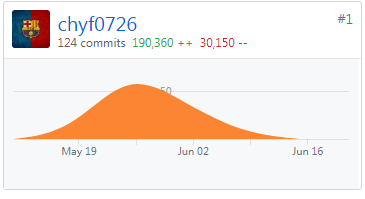
\includegraphics[width=0.7\textwidth]{cyf/contribution.PNG}
	
	We took the advantage of \emph{Github} to promote our cooperation.During the period, I wrote down about 200,000 lines of codes which was mostly written independently,and I was the number 1 contributor in our team.
	
	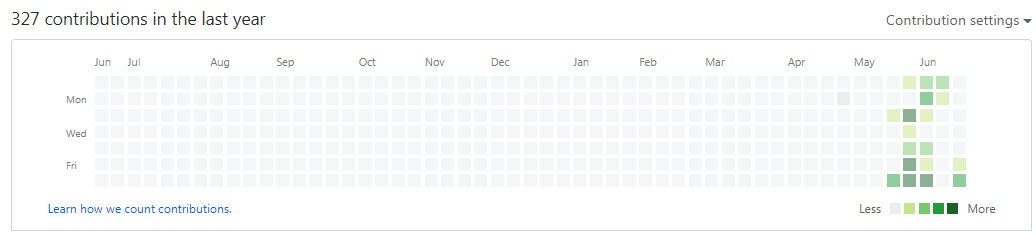
\includegraphics[width=0.7\textwidth]{cyf/frequency.PNG}
	
	I started my job on 26th May and ended on 8th June and I will introduce my job in the following part.
	
	
	\subsection{Index.php}
	
	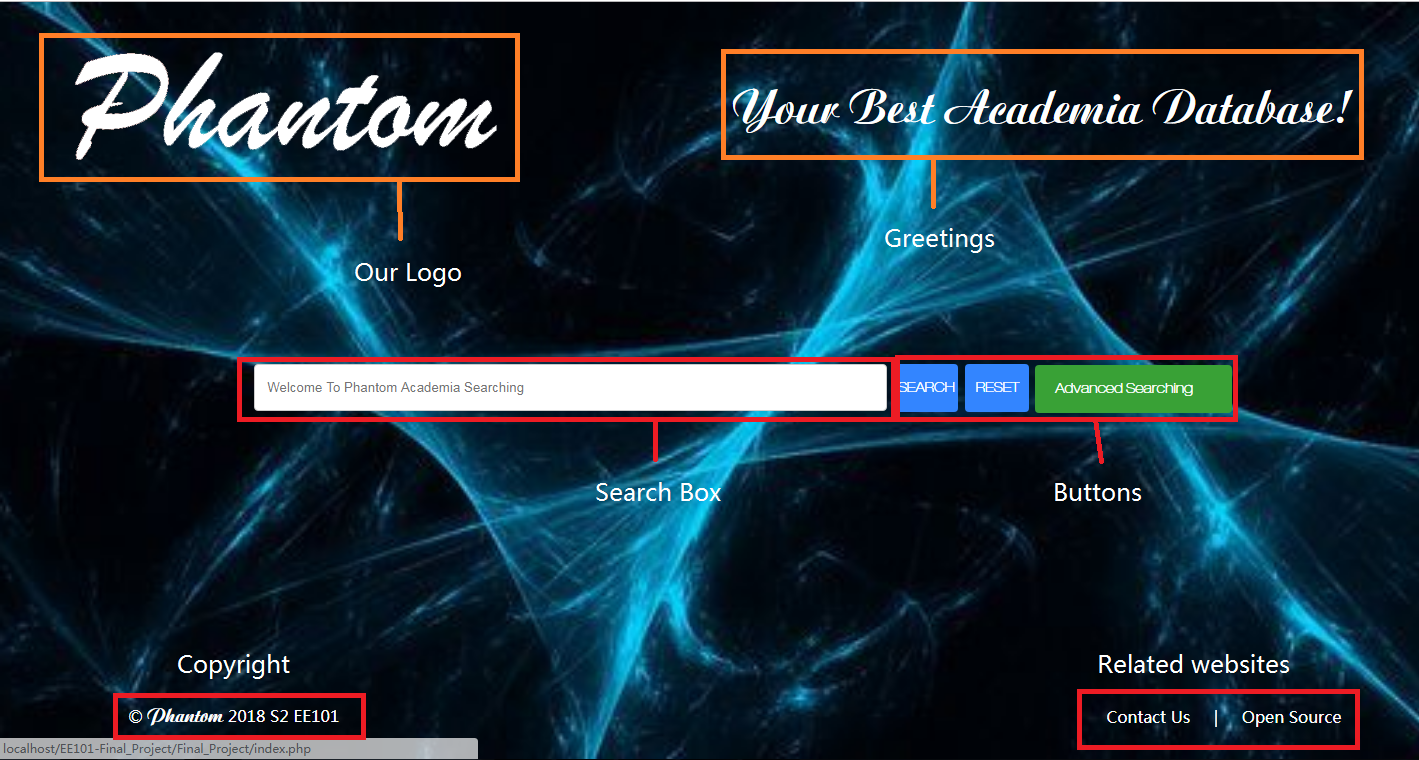
\includegraphics[width=0.7\textwidth]{cyf/index_structure.PNG}
	
	Our index page is shown above.First of all,I would like to introduce the process of my designing our home page.At first,there were three search boxes in the page.The search box "Author","Title" and "conference",and the layout of the index.php was settled.Then,we decided to use multi-searching.Therefore I cut down the number of search boxes into one.Finally,I polished the index.php and the page became what you can see now.
	
	The elements the index page consists of was shown in the graph above,ang I am going to introduce every part respectively.
	
	By the way,the favicon of our websites was \emph{Raffaello}'s \emph{The School of Athens}.
	
	\subsubsection{Logo}
	
	The name of our search engine came from \emph{The Phantom of the opera},one of my favorite films,and I hope that the speed of our searching engine can be as fast as a phantom.It took me so much time to find a appropriate font to display our logo.Finally I found out a font "书体坊兰亭体".However,the words could not be shown in terms of vector graph,which meant that the edge of the words were not smooth,and that is a defect a our logo.
	
	\subsubsection{Greeting Words}
	
	To display the greeting words,I also spent plenty of time to find a approriate fonts.Finally, I found a font named "ChannelSlanted2" to present the greeting words.
	
	\subsubsection{Search box \& buttons}
	
	The search box and the buttons are the key part of the page,and I beautified the buttons,and the result was shown in the following pictures.
	\newline
	\newline
	
\includegraphics[width=0.7\textwidth]{cyf/search1.png}
	\newline
	
\includegraphics[width=0.7\textwidth]{cyf/search2.png}
	\newline
 	
\includegraphics[width=0.7\textwidth]{cyf/search3.png}
 	\newline	
 	
\includegraphics[width=0.7\textwidth]{cyf/search4.png}
 	\newline	
 	
\includegraphics[width=0.7\textwidth]{cyf/search5.png}
 	\newline	
 	
\includegraphics[width=0.7\textwidth]{cyf/search6.png}
 	\newline	
 	
\includegraphics[width=0.7\textwidth]{cyf/search7.png}
 	\newline
	
\includegraphics[width=0.7\textwidth]{cyf/reset1.png}
	\newline
	
\includegraphics[width=0.7\textwidth]{cyf/reset2.png}
	\newline
	
\includegraphics[width=0.7\textwidth]{cyf/reset3.png}
	\newline	
	
\includegraphics[width=0.7\textwidth]{cyf/reset4.png}
	\newline	
	
\includegraphics[width=0.7\textwidth]{cyf/reset5.png}
	\newline	
	
\includegraphics[width=0.7\textwidth]{cyf/reset6.png}
	\newline	
	
\includegraphics[width=0.7\textwidth]{cyf/reset7.png}
	\newline
	
\includegraphics[width=0.7\textwidth]{cyf/Advanced_searching1.png}
	\newline
	
\includegraphics[width=0.7\textwidth]{cyf/Advanced_searching2.png}
	\newline
	
\includegraphics[width=0.7\textwidth]{cyf/Advanced_searching3.png}
	\newline	
	
\includegraphics[width=0.7\textwidth]{cyf/Advanced_searching4.png}
	\newline	
	
\includegraphics[width=0.7\textwidth]{cyf/Advanced_searching5.png}
	\newline	
	
\includegraphics[width=0.7\textwidth]{cyf/Advanced_searching6.png}
	\newline	
	
\includegraphics[width=0.7\textwidth]{cyf/Advanced_searching7.png}
	\newline
	
\includegraphics[width=0.7\textwidth]{cyf/Advanced_searching8.png}
	\newline
	
\includegraphics[width=0.7\textwidth]{cyf/Advanced_searching9.png}
	\newline
	
\includegraphics[width=0.7\textwidth]{cyf/Advanced_searching10.png}
	\newline	
	
\includegraphics[width=0.7\textwidth]{cyf/Advanced_searching11.png}
	\newline	
	
\includegraphics[width=0.7\textwidth]{cyf/Advanced_searching12.png}
	\newline	
	
\includegraphics[width=0.7\textwidth]{cyf/Advanced_searching13.png}
	\newline	
	
\includegraphics[width=0.7\textwidth]{cyf/Advanced_searching14.png}
	\newline	
	
\includegraphics[width=0.7\textwidth]{cyf/Advanced_searching15.png}
	\newline	
	
\includegraphics[width=0.7\textwidth]{cyf/Advanced_searching16.png}
	\newline	
	
\includegraphics[width=0.7\textwidth]{cyf/Advanced_searching17.png}
	\newline	
	
\includegraphics[width=0.7\textwidth]{cyf/Advanced_searching18.png}
	\newline	
	
\includegraphics[width=0.7\textwidth]{cyf/Advanced_searching19.png}
	\newline	
	
\includegraphics[width=0.7\textwidth]{cyf/Advanced_searching20.png}
	\newline	
	
\includegraphics[width=0.7\textwidth]{cyf/Advanced_searching21.png}
	\newline	
	
\includegraphics[width=0.7\textwidth]{cyf/Advanced_searching22.png}
	\newline	
	
\includegraphics[width=0.7\textwidth]{cyf/Advanced_searching23.png}
	\newline	
	
\includegraphics[width=0.7\textwidth]{cyf/Advanced_searching24.png}
	\newline	
	
\includegraphics[width=0.7\textwidth]{cyf/Advanced_searching25.png}
	\newline	
	
\includegraphics[width=0.7\textwidth]{cyf/Advanced_searching26.png}
	\newline	
	
\includegraphics[width=0.7\textwidth]{cyf/Advanced_searching27.png}
	\newline	
	
\includegraphics[width=0.7\textwidth]{cyf/Advanced_searching28.png}
	\newline	
	
\includegraphics[width=0.7\textwidth]{cyf/Advanced_searching29.png}
	\newline	
	
\includegraphics[width=0.7\textwidth]{cyf/Advanced_searching30.png}
	\newline	
	
\includegraphics[width=0.7\textwidth]{cyf/Advanced_searching31.png}
	
	\subsubsection{Copyright \& Related Websites}
	
	These two parts were mainly written by Ziliang Guo and Aofan Jiang and Hyperlinks were set on the texts "Contact Us" and "Open source".
	
	\subsection{Search.php}
	
	I am going to introduce every part of search.php respectively.
	\newline
	
	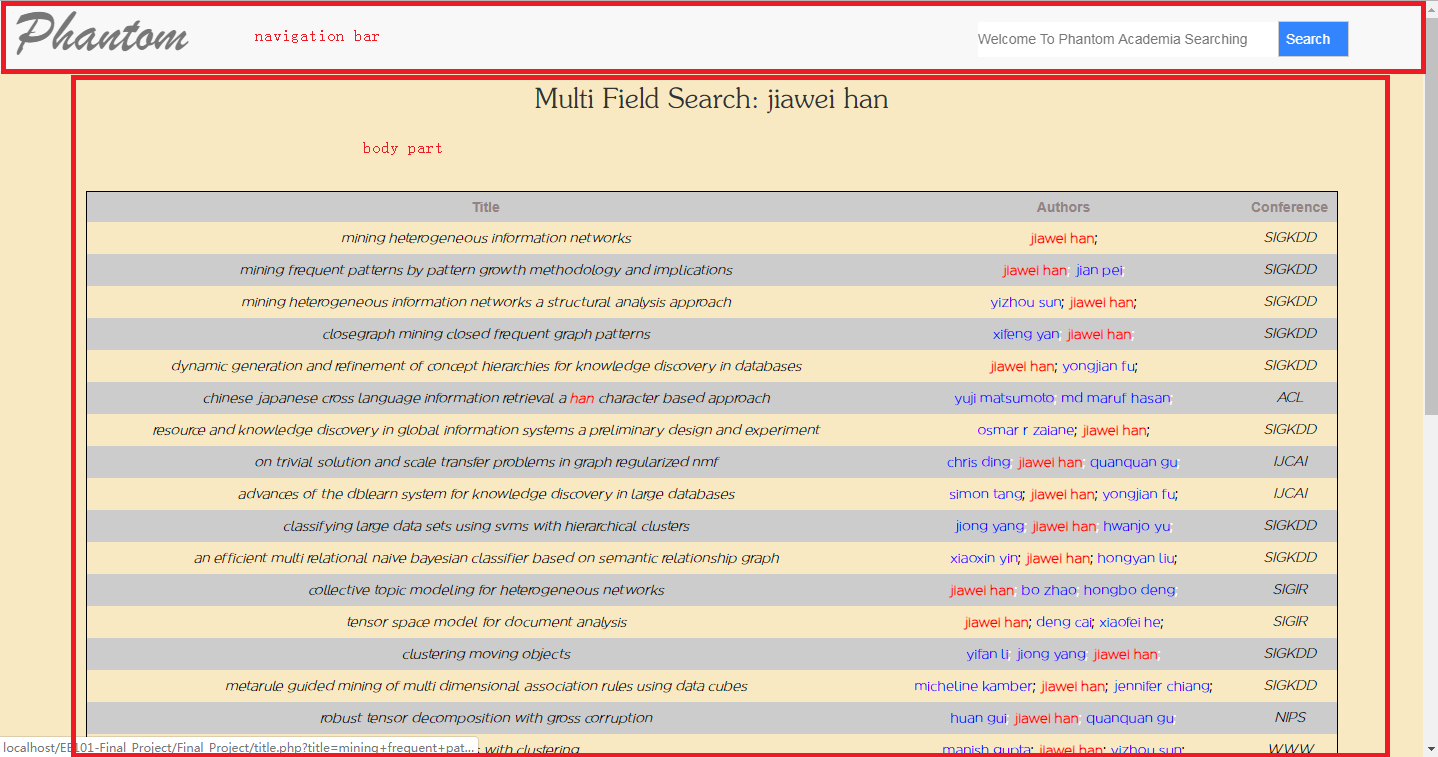
\includegraphics[width=1.0\textwidth]{cyf/SEARCH_struct1.png}
	\newline
	\includegraphics[width=1.0\textwidth]{cyf/SEARCH_2_struct2.png}
	
	
	\subsubsection{Navigation Bar}
	
	I used css and bootstrap to construct the navigation bar.I thought there was no need to build a  that complicated navigation bar,so I just put our logo in the top left corner of the screen and set it with a hyperlink to the homepage,and in the top right corner if the screen was a search box to conduct multi-search.
	
	\subsubsection{Body Part \& Text}
	
	I selected the font "Regencie" to beaufy the table and "书体坊赵九江钢笔楷书" to beatufy the texts.
	
	\subsubsection{Paper Turning \& "Jump to" Button }
	
	Our idea to design the pattern of the Paper Turning is to imitate \emph{Google}'s pattern.
	
	\includegraphics[width=0.5\textwidth]{cyf/Google.jpg}
	
	Therefore,I photoshopped some pictures and realized this idea.
	
	I beautfied the "Jump to" box,and the button "Go!" was modified by Aofan Jiang.
	
	
	\subsection{Conference.php}

 \hspace*{\fill} 
\begin{flushleft}
	\includegraphics[width=1.0\textwidth]{cyf/Conference.PNG}
	\newline
	
	\includegraphics[width=1.0\textwidth]{cyf/Conference2.PNG}
\end{flushleft}

	The beautification of Conference.php was similiar to the search.php.Therefore I will not go into details here.
	
	\subsection{Author.php}
	
	 \hspace*{\fill} 
	\begin{flushleft}
		\includegraphics[width=1.0\textwidth]{cyf/author1.PNG}
		\newline
		
		\includegraphics[width=1.0\textwidth]{cyf/author2.PNG}
	\end{flushleft}

	The beautification of the page author was similiar to the search.php.Therefore I will not go into details here as well.
	
	\subsection{Title.php}
	\begin{flushleft}
		\includegraphics[width=1.0\textwidth]{cyf/Title1.PNG}
		\newline
		
		\includegraphics[width=1.0\textwidth]{cyf/Title2.PNG}
	\end{flushleft}

	I set the texts of the website in a conspicuous position,and the all the texts in the page were shown in selected fonts.I beautified the "Show" button as well.
	
	\subsection{Acknowledgment}
	
	I would like to talk about what I learnt after taking the course \emph{Introduction to Engineering for Electronic Information (B)}.Well,I have to say that this course is a little challenging.The 3 labs and the final projects all covered the fields that I was not familiar with or even never heard about.All these tasks needed me to solve tons of problems and many of them made me mad.However,I got through all these problems with my own effort and the help from my roommates,my classmates and TAs.So here I want to say "Thank You" to all that helped me.I especially want to express my gratitude to TA \emph{Hui Xu}.It was his help and patience that benefited me a lot.I remembered that I met a problem in lab3,and I spent about 4 days solving the problem,but it was still unsolved.Then I turned to TA Xun,and we solved the problem together and finally worked it out.
	
	Then I would like to talk about my work in the final project.As my roommate took the compulsory parts of the final projects,I "had to" do the beautification.I do not think beautification is a job of difficulty,but it required patience.I usually spent plenty of time searching for a awesome fonts and racked my brains to think how can do the webpage better,but when writing this report,I really found it difficult to present my job,for what I have done are only about the layout of the website and some trivial details.I cannot write something like "I used xxx to quicken the search" or "I modified my algorithm with this bright idea".Beautification work is trivial,time-consuming and requires patience but I think I really learn a lot form the work.
	
	Finally,I want to say sorry for my absence of the last course.I do not want to explain anything.The only thing I want to clarify is that I never have any disrespect to Professor Wang and all TAs,and I feel regretful for my absence and apologize sincerely.
	
	Thanks again to all those who have helped me!
	
	
	
	
	
	
	
	
	
	
	
	
		
	
	
	
	
	
	
		
	
	 
	
	
	



% ----------  BEGIN  ------------
% GJL
% ------>	

\newpage

	\section{Graphs}
		\textbf{\emph{[Start] --- By Jialong Guo 518030910272 ---}}\newline\par

	\subsection{Overview}
		\includegraphics[width=0.9\textwidth]{gjl/overview.jpg}\newline\par
		When it comes to our graph part, it can be chiefly divided into three parts: \newline \par
		The first of which is to get all the data we need in order to draw a graph.\newline\par
		The second part of which is to format all the data into the form that the corresponding graph is needed.\newline\par
		The last part of which is just to use specific javascript library to create graphs and make them beautiful. \newline\par

	\subsection{Design}
		\par In author page’s left part, I add a collumn graph, which displays the number of publication the author has yearly and
shows the trend of his/her academic activity to give users a clear impression about the author’s research fruit and the frequency of his/her delivery.
		\par In author page’s left part, I also add a pie graph, which showcases how many papers the author publishs in a conference which brings a clear view on the author is mostly connected with what conference.
		\par In paper page's upper part, there’s a line-collumn graph showing its yearly citations, from which we can gain a insight into the popularity of its research field.
		\par In paper page's lower part, I use a force directed graph to display the relations between similar papers. It gives a convience way to find related papers and messages.
		\par In conference page, a line graph of its yearly amount of papers may reveal its academic influence.

	\subsection{Searching Data}
		\par In this subsection I mainly discuss the first part of graph drawing, get data from database. Since diverse graphs need diverse data, here I just demonstrate a specific example of getting data, which can mostly stand for my means of searching data.
		\subsubsection{From Mysql to Solr}
			\par Taking time cost into consideration, we may need to import data into solr from mysql in advance, for searching from solr will spend more time than from mysql. Thereby, it is required that we write the referenceID of reference papers into solr's schema, which allows us to search the reference papers of a paper just from solr when needed.
			\par The final data we put in solr is formed in this way:\newline\par
			\includegraphics[width=0.9\textwidth]{gjl/formdata.jpg}\newline\par
		You can refer to the codes attached for detailed information.
		\subsubsection{Searching in Solr}
			\par The first step is getting value form user's input, then create the url link to search in solr. After this step, we can get a .json file with the result.

	\subsection{Formatting Data}
		\par In this section, we mainly discuss how to change the search result into suitable formation of drawing a graph. 

	\subsection{Drawing Graph}
		\par In the section, the process of drawing with echarts is mainly discussed.

	\subsection{Fruits' Display}
		\includegraphics[width=0.4\textwidth]{gjl/11.jpg}\newline\par
		\includegraphics[width=0.4\textwidth]{gjl/12.jpg}\newline\par
		\includegraphics[width=0.4\textwidth]{gjl/21.jpg}\newline\par
		\includegraphics[width=0.4\textwidth]{gjl/22.jpg}\newline\par
		\includegraphics[width=0.4\textwidth]{gjl/3.jpg}\newline\par

		\textbf{\emph{[End] --- By Ziliang Guo 518030910273 ---}}

		
% <------
% GJL
% ----------   END   ------------


\newpage


% ----------  BEGIN  ------------
% GZL
% ------>	

	\section{Introduction}
		\textbf{\emph{[Start] --- By Ziliang Guo 518030910273 ---}}\newline\par
		I want to highlight that I greatly emphasize the \textbf{\underline{user-friendliness}} of my work.\par
		(1) I took the initiative that we take full advantage of Github to accelerate our project. I also create a document to take notes of the porblems we met and the solutions.\newline\par
		(2) Actually, I wrote the manual and uploaded my Lab 01 - 03 codes to unify the databases.\newline\par
		(3)	I mainly focus on the back-end development.\newline\par
		(4) Of all my codes, I wanna highlight that approximately 85\% are mainly created \textbf{independently}. For the remaining codes, modification is applied, with reference to some online blogs.\newline\par
		(5) Meanwhile, during my coding, I always remember to leave interfaces for my collaborators.\newline\par
		(6)	As is vividly depicted in the timeline graph, I realized and improved different sections separately, in other words, term by term. Of course, my constant improvements are shown.\newline\par
		\includegraphics[width=0.9\textwidth]{gzl/01.png}

	\newpage

	\section{Keyword Highlighting}
		\emph{Mainly in “search”.}\newline\par
		I adopted the “hl” settings of Solr. It is somehow very simple. Just echo the corresponding urls will do.\par
		However, please notice that, for multivalued fields such as Authors\_Name, only the highlighted part is returned. So I made judgements in such special cases.\par
		Also refer to: http://www.aboutyun.com/thread-9433-1-1.html\newline\par
		Effects:\newline\par
		\includegraphics[width=0.8\textwidth]{gzl/02.png}\newline\par
		Codes:\newline\par
		\includegraphics[width=0.7\textwidth]{gzl/02.jpg}
			%\newline\par
			\newpage
		\includegraphics[width=1\textwidth]{gzl/03.jpg}\par


	\section{Page Turning}
		\emph{In “search”, “author”, “conference”, “advanced search”.}

	\subsection{Brief Introduction}
		Actually, this part undergoes about three versions, and the V1.X version has been discarded because it is too simple.\par
		The features of the versions are:\newline\par
		\includegraphics[width=1\textwidth]{gzl/03.png}\par
		As for the details:\par
		\indent\indent(1) Hyperlink means that I use hyperlinks to jump to a new page.\par
		\indent\indent(2) Anchor refers to the fact that after turning pages, the page will be automatically guided to the titles of the result tables for better user experience.\par
		\indent\indent(3) Jump to stands for the jump-to function, which enables users to jump to a valid page of results.\newline\par
		\indent\indent(4) Actually, the 2.0 and higher version, I tried to imitate the page-turning function of Google. But for the methods, improved hyperlinks for the former, while Jquery and Ajax for the latter.

	\subsection{Details}
	\subsubsection{V1.X}
		This version is just that of my Lab 03 outcomes. It is so simple that only turning to the previous and the next page is availableto users.\newline\par
		Effects:\par
			\indent\indent\includegraphics[width=0.3\textwidth]{gzl/04.png}\par
	\subsubsection{V2.0}
		\emph{In “search”, “author”, “conference”.}\par
		For this version, hyperlinks are used.\newline\par
		As is mentioned above, I try to imitate the page turning function of Google.\par
		In fact, the page number of the current page and the “red-n” above it cannot be clicked and the other numbers and “black-n”s can be clicked, which will direct the user to the corresponding pages.\par
		Meanwhile, when the next page is applicable, the “tom”, the blanked area below, the blanked area to the right and the “Next” can all be clicked. Of course, “Next” appears if and only if the next page exists. It is similar for the previous page, except for the different words (“Pha”, “Prev”).\par
		To implement such function, just create a 2-row table and plug in the corresponding items. Also make judgements whether a page number is the current page. If not, enable cursor and hyperlinks and viceversa.\par
		At first, I wrote a function to calculate the maximum page numebrs using textbf{variable-passing-by-reference}.\par
		Actually, there are altogether four pictures here --- “Pha”, “red-n”, “black-n”, “tom” ---. They are given different file names and CSS features, so it is easy to change images.\newline\par
		%
		I also added the jump-to-page function. To click the “Go” button, a valid number input is reuqired. Otherwise, an error will be raised. The number should be a number greater or equal to 1 and less than or equal to the maximum page number.\par
		If a floating number is inputted, say 1.1 (the same for 1.9), it will be treated as 1. Actually, I am conscious that regular expressions can be adopted here to further ensure the validation. But because of a lack of time, I failed to learn how to use it.\par
		I found "type = number" helpful, but the default up-and-down-arrows confused me a lot. It is ugly and even disgusting!! I found a simple solution using "webkit" of CSS.\par
		Refer to: https://my.oschina.net/qii/blog/341439\newline\par
		Effects:\newline\par
		\includegraphics[width=1\textwidth]{gzl/05.png}\newline\par
		Codes:\newline\par
		\includegraphics[width=1\textwidth]{gzl/04.jpg}
		% \newline\par
		\newpage
		\includegraphics[width=1\textwidth]{gzl/05.jpg}\newline\par
		\includegraphics[width=1\textwidth]{gzl/06.jpg}\newline\par
	\subsubsection{Advanced}
		\emph{In “advanced”.}\par
		For this version, JQuery and Ajax are implemented.\newline\par
		The features are just similar to that of V2.0. It will be introduced later, in section “Advanced Search”.


	\section{Search - Simple and Multi-field}
		\emph{In “search”.}\newline\par
		The simple search V1.0 is just that of my Lab03. It’s simple and sometimes naïve. By the way, some widgets are designed.\newline\par
		%
		For the V2.0, multi-field search is applied. Only one blank is shown. All the results, containing the target keywords in Fields Title, Authors\_Name, and Conference, will be displayed. These fields are of the same importance. Similarly, noinput will lead to an error.\newline\par
		Also refer to:\par
		\indent\indent(1) https://blog.csdn.net/upxiaofeng/article/details/51460042\par
		\indent\indent(2) https://blog.csdn.net/lies\_joker/article/details/51684453\newline\par
		Effects:\newline\par
		\includegraphics[width=0.8\textwidth]{gzl/02.png}\newline\par
		Codes:\newline\par
		\includegraphics[width=0.7\textwidth]{gzl/02.jpg}\newline\par

	\newpage

	\section{Webpage Features}
		\includegraphics[width=1\textwidth]{gzl/06.png}
	\subsection{Refresh}
		For all the pages, after refreshing, the page will jump to the location where the user was previously browsing.\par
		This function is implemented using cookies with reference to: https://www.jb51.net/article/99749.htm\par
		Just include all the body parts in a \emph{<div onscroll=“SetH(this)”>}.\par
		Actually, to a certain extent, I have understood the codes. However, without any hints, I find it hard to do it all on my own.\newline\par
		Codes:\newline\par
		\includegraphics[width=0.75\textwidth]{gzl/07.jpg}
	\subsection{Click Hyperlinks}
		Still, for all the pages, if a hyperlink is clicked, the new page will be opened in a new window.\par
		It is easy to realize using parameter “target="\_blank"”.\newline\par
		Codes:\newline\par
		\includegraphics[width=1\textwidth]{gzl/08.jpg}
	\subsection{Page Turning Anchors}
		It is \textbf{absolutely extremely disgusting} to be not guided to the head of the result table while turning pages!\par
		Therefore, at the beginning of each result table, I set a anchor, which is added into the hyperlinks.\newline\par
		Codes:\newline\par
		\includegraphics[width=1\textwidth]{gzl/09.jpg}
	\subsection{Loading Speed Improvements}
		In addition, I improved the loading speed of the author page.\par
		Originally, a request will be delivered to MySQL to search the most related affiliation. However, such a process is actually unnecessary at all!\par
		So I pass the most related affiliation name while turning pages. The outcome is apparent!

	\section{Paper Recommendation}
		Ten recommended papers in academic formats, which can be hidden and shown, is available on the title page.\par
		\includegraphics[width=1\textwidth]{gzl/07.png}\par
		The order and weight account for three parameters. Cited times are given top priority, followed by authors and title. The authors of a certain paper are given a descending weight and the weight of the title is similar to that of the first author.\newline\par
		%
		The implementation is similar to that of the multi-field search, except that in this case, different parameters are assigned varied weight.\par
		Notice that:\par
		\indent\indent(1) The recommended papers can be clicked to acquire a deeper insight.\par
		\indent\indent(2) Few groups pay attention to the \textbf{academic format of paper information}.\newline\par
		%
		Actually, the hide-and-show process is very very \textbf{fluent}!\par
		To implement such function, I adopted JavaScript with reference to:\par
		\indent\indent https://blog.csdn.net/baidu\_35701759/article/details/76187236\par
		It helps a lot at the beginning.\newline\par
		%
		Effects:\newline\par
		\includegraphics[width=1\textwidth]{gzl/10.jpg}\newline\par
		%
		Codes:\newline\par
		\includegraphics[width=0.9\textwidth]{gzl/11.jpg}

	\newpage

	\section{Advanced Search}
	\subsection{Overview}
		\begin{large}\underline{\textbf{The advanced search is key to a good search engine!}}\end{large}\newline\par
		\includegraphics[width=1\textwidth]{gzl/14.jpg}\newline\par
		Here, we may reach some agreements on the names:\par
		\indent\indent(1) The area with the key word boxes is called: Search Bar;\par
		\indent\indent(2) The empty area now in yellow is called: Result Area.\par
		This page is made separately using mianly Jquery. I was also in charge of \textbf{most of its front-end coding}.\par
		For this part, since the unclarity and difficulty of division, I recommend that if you are interesting in the codes, please have a look at the source codes attached. I will point out the exact file names.\par
		The main page (default file) is “\underline{index\_search\_advanced.php}”.
	\subsection{Search Bar}
		Apparently, the “+” and “-” are bound to different incidents, which will send requests to “\underline{07\_advanced\_search\_boxes.php}” to update the number of boxes.\par
		For the bool part, users can choose \emph{And} or \emph{Or}.\par
		For the target part, users can choose \emph{Title}, \emph{Author} or \emph{Conference}.
		Foe the input part, users can input anything. Phrases with spaces are also ok.
		There are some \textbf{details worth consideration}:\par
		(1) After clicking the add-or-delete buttons, the filled values must be kept. Therefore, while requesting, the url contains all the values of the existing items. The approach is simple, just get the values according to the id and sequence them. Then, in the php file, GET these values and set it as the default values.\par
		(2) When there is only one line, the “-” button must be hidden. Just change the display mode while updating the “innerHTML” content.\par
		(3) Check for unfilled blanks and alert if exists when the search button is clicked. Loop works well. But attention must be paid to some small aspects.\par
		(4) When there are too many lines, how should it appears? Actually, “overflow-y=auto” will do.\par
		(5) Take care if there are spaces in the values! String replacement is required.\par
		(6) Absolutely, for the first line, boolean selection is unnecessary. Thus, for both directions - add to two rows, delete to one row - deserves carefulness.\newline\par
		%
		Effects:\newline\par
		\includegraphics[width=0.5\textwidth]{gzl/10.png}
	
	\subsection{Submit}
		After clicking the submit button, the parameters will be contained in the request, and the results will be shown in the Result Area.\par
		It is a multi-field search. The keywords are given a slowly descending weight.\par
		When clicked, a request containing all the parameters is sent to\newline“\underline{07\_search\_advanced.php}”. The codes there are similar to that of “search” page.\par
		Then, the reults are loaded.\par
		But the page turning area is loaded with he function “turn\_page()”, where maximum and minimum page numbers are calculated and a request, containing the target page number, is sent to “\underline{07\_advanced\_search\_pages}”.
		Please notice that, I am greatly anxious about the user-friendliness. Therefore, I made it a rule that every successfull search will lead to the fact that the Search Bar \textbf{gradually slides and hides}. When it is hidden, a bar is for calling it back and viceversa. Of course, at first, this call-back-bar can not be seen. Here, the main part is similar to that of the paper recommendation hide-and-show of the “title” page, except for some details. You may refer to “07\_show\_hide.js”.\newline\par
		Effects:\newline\par
		\includegraphics[width=0.9\textwidth]{gzl/15.jpg}

	\subsection{Page Turning and Jump-to}
		Firstly, page turning codes in “\underline{07\_advanced\_search\_pages.php}”:\par
		Similar to the traditional page turning functions, show the numbers and the images. But here, the images are bound with “onclick()” functions instead of hyperlinks. For the numbers, the hyperlink is bound with a “onclick(submit\_search(\$new\_page,1))” function and must not be jumped to “href”. Thus, this approach works:\par
		\indent\indent href="\#" onclick="submit\_search(\$new\_page,1); return false;"\par
		Also refer to:\par
		\indent\indent https://blog.csdn.net/fendou123\_love/article/details/53585016\newline\par
		%
		Secondly, “submit\_search(page,1)” in “\underline{index\_advanced\_search.php}”:\par
		Turing pages are just the same as submitting a search request, except for the fact that the former requires the search bar always being kept hidden and the latter being changed from visible to invisible. Therefore, I need a parameter to indicate such difference(1 for turning pages, 0 for submits).\newline\par
		%
		Thirdly, jump-to function in “\underline{07\_advanced\_search\_pages.php}”:\par
		The main codes are similar to those of the traditional search. But here, the JUMP button is bound with “onclick=jump\_to\_submit()” instead of a hyperlink.\newline\par
		%
		Fourthly, “jump\_to\_submit()” in “\underline{index\_advanced\_search.php}”:\par
		The validation (i.e. filled/unfilled, maximum, minimum) of the inputted target page number is checked first. If it not valid, alert the error. Then, just the same as turning pages, call “submit\_search(new\_page,1);”\newline\par
		%
		Effects:\newline\par
		\includegraphics[width=1\textwidth]{gzl/16.jpg}

	\newpage

	\section{Feedback}
		We value users’ precious feedbacks. So we add a feedback page.\par
		We are curious about four fields: the user's name, the e-mail address, the subject and what we can do for the user. Therefore, four blanks are required. The unfilled blanks will be alerted and the pending status will be clearly illustrated.\par
		\indent\indent\includegraphics[width=0.35\textwidth]{gzl/08.png}\newline\par
		%
		What’s more, the log will be saved locally in a clear enough format.\par
		\indent\indent\includegraphics[width=0.65\textwidth]{gzl/09.png}\newline\par
		%
		Although PHPMailer seems to be much more convenient, something wrong occurred such as missing an authentic certificate. In the end, such approach was discarded.I take advantage of NodeJS and emailjs to implement the function.\par
		Still, I mainly use JQeury to implement this section. When clicked, the valid messages will be connected together and passed to the requested .php file, where the cmd console will be run (using “exec()”) to call the nodejs mail-sending function.\newline\par
		%
		Reference:\par
		\indent\indent(1) HTML - send e-mails: http://www.fly63.com/article/detial/620\par
		\indent\indent(2) PHP - exce(): https://blog.csdn.net/sinat\_29862853/article/details/85253384\par
		\indent\indent(3) PHP - get system time: https://www.jb51.net/article/148361.htm\par
		\indent\indent(4) PHP - file read: https://www.cnblogs.com/penghuwan/p/6884932.html\par
		\indent\indent(5) PHP - file read: https://www.cnblogs.com/penghuwan/p/6884932.html\par
		\indent\indent(6) NodeJS - run with given parameters:\par
			\indent\indent\indent https://www.jianshu.com/p/474e6d76f867\par
			\indent\indent\indent https://cloud.tencent.com/developer/article/1363526\newline\par
		%
		\newpage
		Codes:\newline\par
		\includegraphics[width=0.9\textwidth]{gzl/12.jpg}\newline\par
		\includegraphics[width=0.9\textwidth]{gzl/13.jpg}\newline\par

	\textbf{\emph{[End] --- By Ziliang Guo 518030910273 ---}}
% <------
% GZL
% ----------   END   ------------

\newpage

% ----------  BEGIN  ------------
% JAF
% ------>	

\section{Hyperlinks}
\textbf{\emph{--- By Aofan Jiang 518030910275 ---}}\newline\par
As required in the final project, I add the hyperlink of each title, author and conference. So the users can click to get more information about the result they want to search for.
\subsection{Hyperlink of each title}
Different from the table about the information of key words, the title page is simply a series of main information about the corresponding paper. It includes the paper ID, the publish year, the authors, conference name, and reference papers. This can make the whole page clearer,just as the following picture.\newline\par
\includegraphics[width=0.9\textwidth]{jaf/titleexample.PNG}\newline\par
 It might be ignored that the table of reference paper title of each paper is given in the original data. Although it is not required in the lab two, I still add it as a field in Solr to make sure that more detailed information can be gotten by the users. This explains the existence of references in the paper page.\newline\par
What’s more, to make a user-friendly website, you can see in the following picture that at the top of website, the link information about the title. It’s also clear and easy to find the information. It’s linked by the symbol of addition.\par
\includegraphics[width=0.9\textwidth]{jaf/link.PNG}\newline\par
 On the comparison, you can see even in Baidu NetDisk that the link is not so comfortable as ours. They are all connected with \%2 while our website link are connected with + . Since all the information is imported in solr, the searching speed is quite fast with no delay.\par
\includegraphics[width=0.9\textwidth]{jaf/linked.PNG}\newline\par
\subsection{Hyperlink of each conference}
This page is also mainly an information table like the main searching page. It includes each paper’s title, authors published on the given conference name. However, at the last column of table, the original conference name is replaced by the publish year of each paper published in this conference.\par
\includegraphics[width=0.9\textwidth]{jaf/conference.PNG}\newline\par
\subsection{others}
Even at different pages among paper, author, conferences. Almost all the items are hyperlinked. So it means you can jump to different pages in any given page. Here comes an example of authors' information\par
\includegraphics[width=0.9\textwidth]{jaf/author.PNG}\par

\section{Code optimization}
\subsection{Solr}
By testing, I find that the searching speed by solr is faster than mysql. So all the places that can be used in solr are changed from mysql.\par
\subsection{Mysql}
When using mysql, there are still some methods to improve the speed of program.\par If the searching result is only one piece. For instance, the publish year, the affiliation and the conference and so on. We can limit the searching result numbers by add the code “LIMIT 1 ”. As a result, when mysql get one information about the result, it will stop the searching process, which is a great improvement in the speed of a program.\par
\includegraphics[width=0.9\textwidth]{jaf/limit.PNG}\newline\par
 Instead of using inner join, try to use more simple searching and output the result together is faster.\par
\includegraphics[width=0.9\textwidth]{jaf/affold.PNG}\newline\par
\includegraphics[width=0.9\textwidth]{jaf/affnew.PNG}\newline\par
As for the code in php, we can choose to use mysqli\_fetch\_row rather than mysqli\_fetch\_array since the information class is of each column is known to us.\par

\section{Contact and Open source}
At the home page, you can find the word “contact us ”. After clicking it, you will jump to a new page with a sophisticated chart. You can input your information and your information, we will get your feedback after you clicking the submit button.\newline\par
\includegraphics[width=0.9\textwidth]{jaf/contact.PNG}\newline\par
Also, you can find the word ”open source ”. After clicking it, you will jump to our project on Github website. At here, you can check all the detailed codes and corresponding documents.\newline\par
\includegraphics[width=0.9\textwidth]{jaf/git.PNG}\newline\par
\newpage

% <------
% JAF
% ----------   END   ------------




\end{document}